\documentclass[12pt,letterpaper]{article}
\usepackage{graphicx,textcomp}
\usepackage{natbib}
\usepackage{setspace}
\usepackage{fullpage}
\usepackage{color}
\usepackage[reqno]{amsmath}
\usepackage{amsthm}
\usepackage{fancyvrb}
\usepackage{amssymb,enumerate}
\usepackage[all]{xy}
\usepackage{endnotes}
\usepackage{lscape}
\newtheorem{com}{Comment}
\usepackage{float}
\usepackage{hyperref}
\newtheorem{lem} {Lemma}
\newtheorem{prop}{Proposition}
\newtheorem{thm}{Theorem}
\newtheorem{defn}{Definition}
\newtheorem{cor}{Corollary}
\newtheorem{obs}{Observation}
\usepackage[compact]{titlesec}
\usepackage{dcolumn}
\usepackage{tikz}
\usetikzlibrary{arrows}
\usepackage{multirow}
\usepackage{xcolor}
\newcolumntype{.}{D{.}{.}{-1}}
\newcolumntype{d}[1]{D{.}{.}{#1}}
\definecolor{light-gray}{gray}{0.65}
\usepackage{url}
\usepackage{listings}
\usepackage{color}
\usepackage{verbatim} % includes comment blocks

\definecolor{codegreen}{rgb}{0,0.6,0}
\definecolor{codegray}{rgb}{0.5,0.5,0.5}
\definecolor{codepurple}{rgb}{0.58,0,0.82}
\definecolor{backcolour}{rgb}{0.95,0.95,0.92}

\lstdefinestyle{mystyle}{
	backgroundcolor=\color{backcolour},   
	commentstyle=\color{codegreen},
	keywordstyle=\color{magenta},
	numberstyle=\tiny\color{codegray},
	stringstyle=\color{codepurple},
	basicstyle=\footnotesize,
	breakatwhitespace=false,         
	breaklines=true,                 
	captionpos=b,                    
	keepspaces=true,                 
	numbers=left,                    
	numbersep=5pt,                  
	showspaces=false,                
	showstringspaces=false,
	showtabs=false,                  
	tabsize=2
}
\lstset{style=mystyle}
\newcommand{\Sref}[1]{Section~\ref{#1}}
\newtheorem{hyp}{Hypothesis}



% Title Page
\title{House Price Prediction}
\author{Team B}


\begin{document}
\maketitle



%\section*{Data Description}
%code book

%\section{Data Wrangling}

%\section{Prediction}
% Table created by stargazer v.5.2.3 by Marek Hlavac, Social Policy Institute. E-mail: marek.hlavac at gmail.com
% Date and time: Wed, Nov 16, 2022 - 14:17:52
\begin{table}[!htbp] \centering 
  \caption{} 
  \label{} 
\begin{tabular}{@{\extracolsep{5pt}}lcc} 
\\[-1.8ex]\hline 
\hline \\[-1.8ex] 
 & \multicolumn{2}{c}{\textit{Dependent variable:}} \\ 
\cline{2-3} 
\\[-1.8ex] & \multicolumn{2}{c}{AdjSalePrice} \\ 
\\[-1.8ex] & (1) & (2)\\ 
\hline \\[-1.8ex] 
 SqFtTotLiving & 202.766$^{***}$ & 202.906$^{***}$ \\ 
  & (2.877) & (2.857) \\ 
  & & \\ 
 BldgGrade & 97,573.830$^{***}$ & 94,901.400$^{***}$ \\ 
  & (2,227.820) & (2,217.296) \\ 
  & & \\ 
 ZipGroup & 79,521.530$^{***}$ &  \\ 
  & (1,142.365) &  \\ 
  & & \\ 
 as.factor(ZipGroup)2 &  & 50,292.380$^{***}$ \\ 
  &  & (5,716.560) \\ 
  & & \\ 
 as.factor(ZipGroup)3 &  & 108,101.700$^{***}$ \\ 
  &  & (5,019.663) \\ 
  & & \\ 
 as.factor(ZipGroup)4 &  & 174,629.400$^{***}$ \\ 
  &  & (5,340.195) \\ 
  & & \\ 
 as.factor(ZipGroup)5 &  & 327,892.000$^{***}$ \\ 
  &  & (4,898.939) \\ 
  & & \\ 
 Constant & $-$852,923.100$^{***}$ & $-$729,031.600$^{***}$ \\ 
  & (13,351.420) & (13,436.110) \\ 
  & & \\ 
\hline \\[-1.8ex] 
Observations & 20,340 & 20,340 \\ 
R$^{2}$ & 0.622 & 0.628 \\ 
Adjusted R$^{2}$ & 0.622 & 0.627 \\ 
Residual Std. Error & 238,138.700 (df = 20336) & 236,376.200 (df = 20333) \\ 
F Statistic & 11,148.740$^{***}$ (df = 3; 20336) & 5,709.036$^{***}$ (df = 6; 20333) \\ 
\hline 
\hline \\[-1.8ex] 
\textit{Note:}  & \multicolumn{2}{r}{$^{*}$p$<$0.1; $^{**}$p$<$0.05; $^{***}$p$<$0.01} \\ 
\end{tabular} 
\end{table} 


	\begin{figure}
		  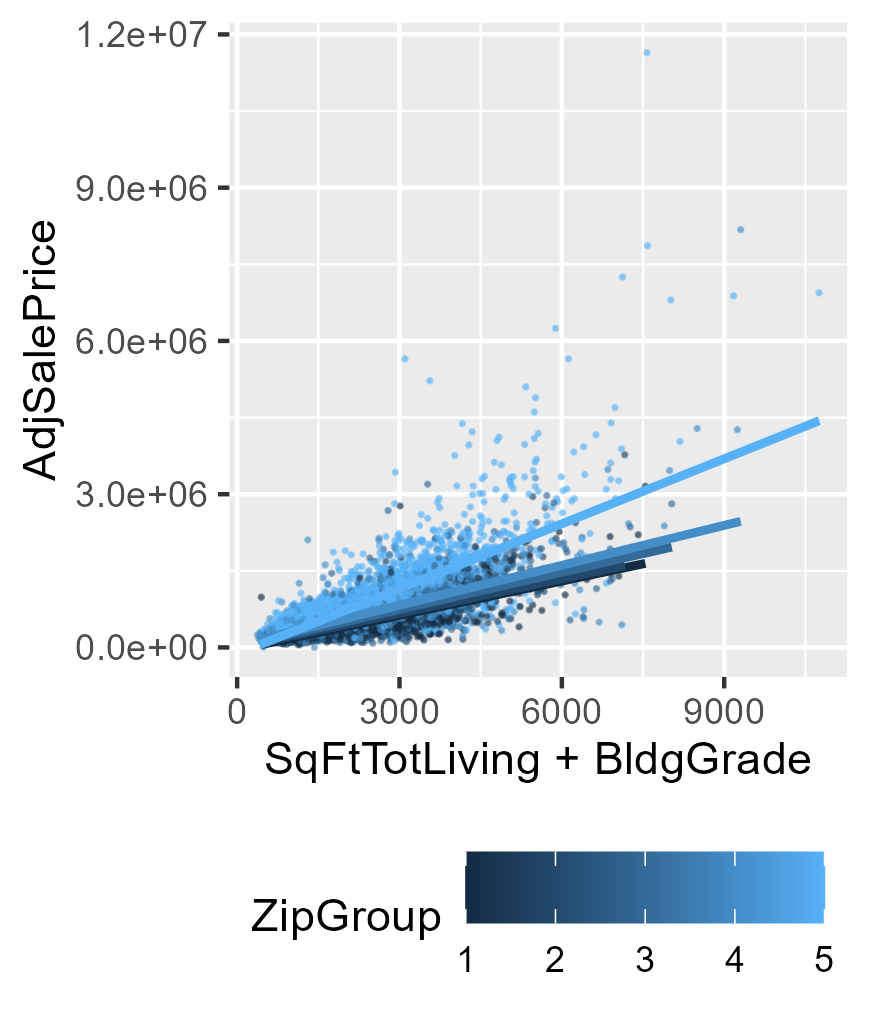
\includegraphics[width=0.9\textwidth]{ZipGroup.png}
		  \caption{using building grade, living space and clustered ZipCode to predict house prices }
		  
	\end{figure}


	\begin{figure}
		  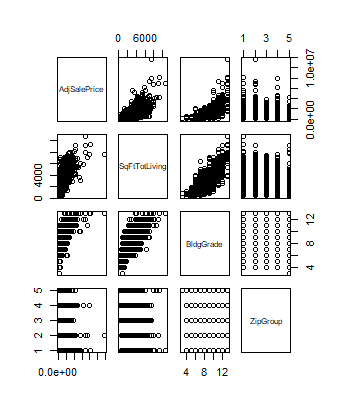
\includegraphics[width=0.9\textwidth]{model_pairs.png}
		  \caption{using building grade living space and ZipCode to predict house prices }
		  
	\end{figure}


\end{document}          
